\section{Topic Centrality}\label{sec:TopicCentrality}

As outlined in section \ref{sec:TopicModellingRes}, seven salient topics were
extracted from the corpus of party leader tweets. To reiterate, these topics can
be labeled as: 1) campaign dynamics, 2) carbon tax, 3) SNC Lavalin, 4) middle
class appeals, 5) celebratory messages, 6) diversity and immigration, and 7)
healthcare. After introducing the engagement graph defined in section
\ref{ch:GraphTheory}, and the concept of eigenvector centrality (section
\ref{sec:EigCentrality}), measures of topic centrality can be explored. In order
to achieve the secondary objective of measuring what topics rally, and what
topics span, party leaders' bases two measures of topic centrality have been
developed: total network topic centrality and party leader topic centrality. By
juxtaposing the two, various insights about how different topics influenced
discourse can be derived.

\subsection{Total Network Topic Centrality}\label{sec:NetTopicCentrality}

\begin{singlespacing}
    \begin{figure}[H]
    \centering
    \includegraphics[scale=0.15]{Figures/og_graph}
    \caption[Complete Political Engagement Graph]{Complete Political Engagement Graph}
    \label{fig:og_graph_copy}
    \end{figure}
\end{singlespacing}

Total network topic centrality is an aggregate of the eigenvector centrality of
all tweets of a certain topic in the entire engagement graph. For reference,
this graph has been reproduced in figure \ref{fig:og_graph_copy}. More formally,
and with slight abuse of notation, the total network topic centrality of topic
$i$, $T_{i}$, can be defined as the set of all eigenvector centrality measures for tweet
vertices of topic $i$ in a graph $G$. 

\begin{equation}
    T_{i} := \{ C_{E}(x) , \forall x \in G \mid type(x)=tweet, topic(x)=i \}
\end{equation}

When taking the aggregate (sum, mean, z-score relative to other topics), a
single number can be assigned to the relative importance of topic $i$. And in
keeping with the strengths of eigenvector centrality, $T_{i}$ will be larger if:
those tweets are retweeted a lot, and if they're retweeted by \emph{highly
engaged} users.

\subsection{Party Leader Topic Centrality}\label{sec:LeaderCentrality}

In order to measure how central a topic is to a party leader's base, party
leader topic centrality was developed. This assumes a world in which party
leader $j$ is the only actor with which generic users can engage with. This is
done by taking a subgraph of $G$ -- $G_{j}$ -- which only contains party leader
$j$, all of $j$'s tweets, $X$, and all edges from $x\in X$ to the generic users
who retweeted one of $j$'s tweets. An example of this is in figure
\ref{fig:jagmeet_singh_subgraph}, which demonstrates the subgraph for Jagmeet
Singh. 

After the subgraph $G_j$ is constructed, the party leader topic
centrality $P_{ij}$ is defined as the set of all eigenvector centrality measures
for tweet vertices of topic $i$ in a graph $G_{j}$.

\begin{equation}
    P_{ij} := \{ C_{E}(x) ,  \forall x \in G_{j} \mid type(x)=tweet, topic(x)=i \}
\end{equation}

\begin{singlespacing}
    \begin{figure}[H]
    \centering
    \includegraphics[scale=0.15]{Figures/jagmeet_singh_subgraph}
    \caption[Political Engagement Subgraph for Jagmeet Singh]{Political Engagement Subgraph for Jagmeet Singh}
    \label{fig:jagmeet_singh_subgraph}
    \end{figure}
\end{singlespacing}

\subsection{Results}\label{sec:TopicCentralityResults}

After calculating $\textbf{T}=\{T_{i} \mid \forall i \in
topics\}$\footnote{$topics$ refers to the seven topics that tweets were labelled
as in section \ref{sec:TopicModellingRes}.} and $\textbf{P}=\{P_{ij} \mid
\forall i \in topics,\forall j \in party\_leaders\}$\footnote{$party\_leaders$
refers to the five Canadian Federal party leaders referred to in section
\ref{sec:motivation}.}, each individual centrality measure, $T_{i} \in
\textbf{T}$ and $P_{ij}\in \textbf{P}$, can be summated
($\hat{T_{i}}$/$\hat{P_{ij}}$), have it's mean calculated
($\overline{T}_{i}$/$\overline{P}_{ij}$), or have it's z-score taken relative to
other topics in its set\footnote{For the party leader topic centrality, the
z-score of topic centrality is based off of other tweet topics for that party
leader.} ($\stackrel{z}{T}_{i}$/$\stackrel{z}{P}_{ij}$).

Figure \ref{fig:topic_centrality} shows plots of $\textbf{T}$ as a function of
$\textbf{P}$, each point is coloured according to its party leader and is
annotated with the topic that it pertains to. The x-axis is the party leader
topic centrality score for all party leader and topic combinations -- and the y-axis
is the total network topic centrality score for each topic\footnote{This
explains why all party leader topic centrality scores for the same topic lie on
the same point on the y-axis.}.

\begin{singlespacing}
    \begin{figure}
        \centering
        \begin{tabular}{ccc}
        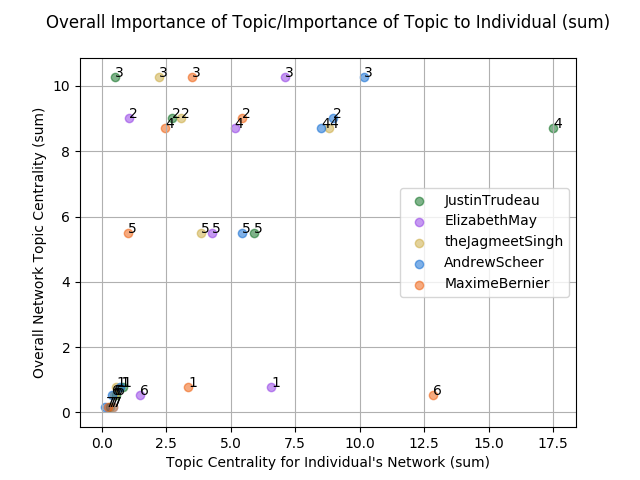
\includegraphics[width=50mm]{Figures/sum_opposing_centrality_chart_(expanded)} &
        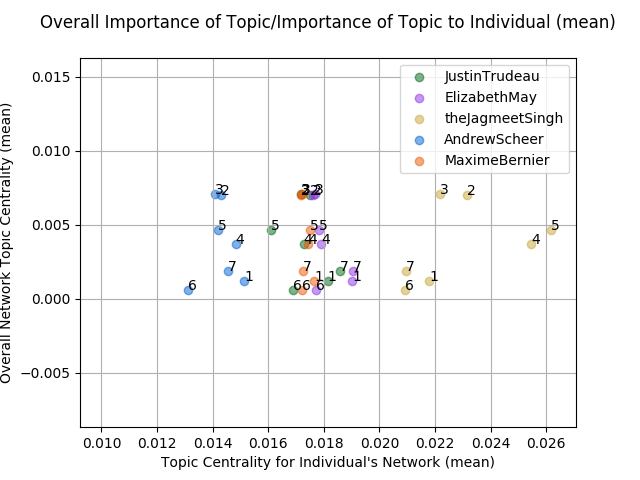
\includegraphics[width=50mm]{Figures/mean_opposing_centrality_chart_(expanded)} &
        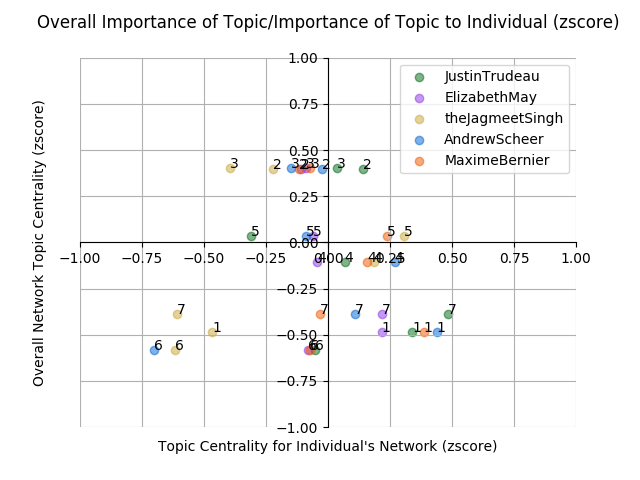
\includegraphics[width=50mm]{Figures/zscore_opposing_centrality_chart_(expanded)} \\
        (a)  \textbf{$\hat{T}$} by \textbf{$\hat{P}$} & \textbf{$\overline{T}$} by \textbf{$\overline{P}$} &  \textbf{$\stackrel{z}{T}$} by \textbf{$\stackrel{z}{P}$} \\[6pt]
        \end{tabular}
        \caption[$\textbf{T}$ aggregates in relation to $\textbf{P}$]{$\textbf{T}$ aggregates in relation to $\textbf{P}$}
        \label{fig:topic_centrality}
    \end{figure}
\end{singlespacing}

Some initial insights from comparing \textbf{$\hat{T}$} by \textbf{$\hat{P}$}
with \textbf{$\overline{T}$} by \textbf{$\overline{P}$}; while Maxime Bernier
promoted a large number of tweets regarding immigration, free speech and
diversity as indicated by a high $\hat{P}_{6M}$ -- these tweets gained little
traction overall in the entire network ($\stackrel{z}{T_{6}}$) as well as
compared to other topics Bernier tweeted about $\stackrel{z}{P}_{6M}$.
Additionally, despite the relatively few tweets pertaining to health care and
pharmacare (topic 7), and the low total network centrality score
($\stackrel{z}{T_{7}}$), they were disproportionately important to Justin
Trudeau's network ($\stackrel{z}{P}_{7T}$). Discrepancies in a topic that gives
the highest $\hat{P_{ij}}$ for a party leader (total topic engagement) and
$\overline{P}_{ij}$  (mean topic engagement) can illustrate inefficiencies in
connecting with their target demographic.

As well, for each topic -- the party leader topic centrality score can be
averaged across all the different party leaders to give a more general analysis
of how central topics were to the entire network, or to any individual party
leader. This is shown in figure \ref{fig:topic_centrality_combined}. Here it is
most insightful to look at \textbf{$\stackrel{z}{T}$} by
\textbf{$\stackrel{z}{P}$}, specifically in the lower right-hand quadrant and
upper left-hand quadrant. The former indicates tweet topics that are more
important to a party leader's base than to the entire network (topics 7 and 1).
Topic 1 -- campaign dynamics -- intuitively makes sense in this category; it is
not surprising that messages about the campaign, where rallies are, etc... would
appeal more to a party leader's base than to the entire network. Conversely,
tweets in the upper left-hand quadrant indicates tweet topics that are more
important to the overall network than to the individual network -- which may be
an indication of those topics spanning partisan divides (topics 2 and 3).

\begin{singlespacing}
    \begin{figure}
        \centering
        \begin{tabular}{ccc}
        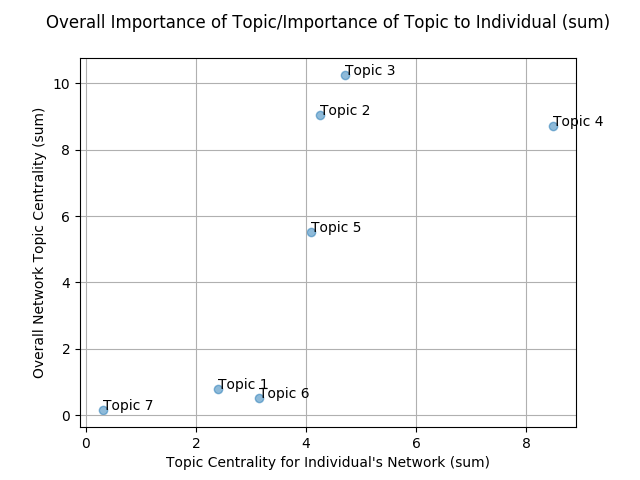
\includegraphics[width=50mm]{Figures/sum_opposing_centrality_chart_(mean_of_leaders)} &
        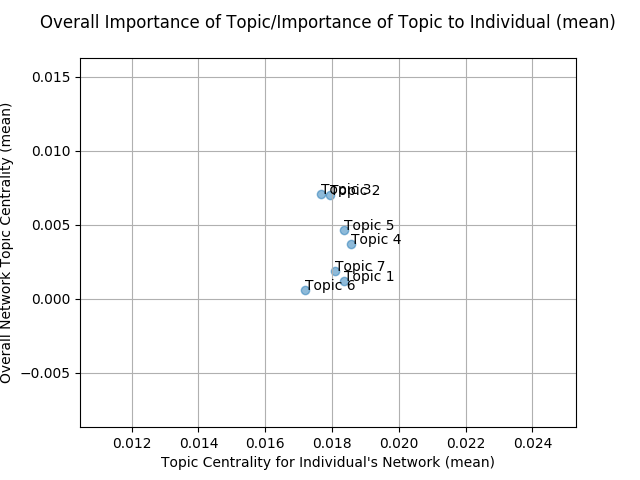
\includegraphics[width=50mm]{Figures/mean_opposing_centrality_chart_(mean_of_leaders)} &
        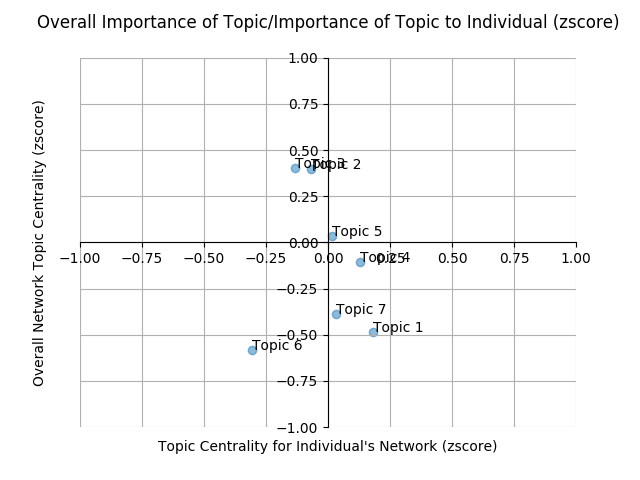
\includegraphics[width=50mm]{Figures/zscore_opposing_centrality_chart_(mean_of_leaders)} \\
        (a)  \textbf{$\hat{T}$} by \textbf{$\hat{P}$} & \textbf{$\overline{T}$} by \textbf{$\overline{P}$} &  \textbf{$\stackrel{z}{T}$} by \textbf{$\stackrel{z}{P}$} \\[6pt]
        \end{tabular}
        \caption[$\textbf{T}$ aggregates in relation to $\textbf{P}$ (party leader average)]{$\textbf{T}$ aggregates in relation to $\textbf{P}$ (party leader average)}
        \label{fig:topic_centrality_combined}
    \end{figure}
\end{singlespacing}

\begin{singlespacing}
\begin{center}
    \begin{threeparttable}
    \caption{Topic Centrality Measure Results}
    \label{fig:tab_topic_cent_results}\begin{small}
        \begin{tabular}{|l|c|c|c|c|c|c|c|c|c|} \hline
        \multicolumn{1}{|c|}{}  & \multicolumn{3}{|c|}{\specialcell{Total Network\\Topic Centrality}} & \multicolumn{3}{|c|}{\specialcell{Andrew\\Scheer}} & \multicolumn{3}{|c|}{\specialcell{Elizabeth\\May}} \\ 
        \hline
        Topic                   & \textbf{$\hat{T}$} & \textbf{$\overline{T}$} & \textbf{$\stackrel{z}{T}$} & \textbf{$\hat{P}$} & \textbf{$\overline{P}$} & \textbf{$\stackrel{z}{P}$}& \textbf{$\hat{P}$} & \textbf{$\overline{P}$} & \textbf{$\stackrel{z}{P}$}\\
        \hline
        1 & 0.779   & 0.001 & -0.486    & 0.726     & \textbf{0.015} & \textbf{0.438}     & \textbf{6.566} & \textbf{0.019} & 0.216     \\  
        \hline
        2 & 9.034   & \textbf{0.007} & 0.395     & 8.947     & 0.014 & -0.024    & 1.074 & 0.017 & -0.110    \\  
        \hline
        3 & \textbf{10.263}  & \textbf{0.007} & \textbf{0.402}     & \textbf{10.176}    & 0.014 & -0.148    & 7.097 & 0.018 & -0.090    \\ 
        \hline
        4 & 8.719   & 0.004 & -0.106    & 8.500     & \textbf{0.015} & 0.269     & 5.156 & 0.018 & -0.043    \\ 
        \hline
        5 & 5.507   & 0.005 & 0.033     & 5.425     & 0.014 & -0.088    & 4.278 & 0.018 & -0.061    \\  
        \hline
        6 & 0.519   & 0.001 & -0.580    & 0.380     & 0.013 & -0.703    & 1.490 & 0.018 & -0.082    \\ 
        \hline
        7 & 0.153   & 0.002 & -0.387    & 0.145     & \textbf{0.015} & 0.107     & 0.438 & \textbf{0.019} & \textbf{0.218}     \\ 
        \hline
        \multicolumn{1}{|c|}{}  & \multicolumn{3}{|c|}{\specialcell{Jagmeet\\Singh}} &\multicolumn{3}{|c|}{\specialcell{Justin\\Trudeau}} &\multicolumn{3}{|c|}{\specialcell{Maxime\\Bernier}} \\\hline
        Topic                   & \textbf{$\hat{P}$} & \textbf{$\overline{P}$} & \textbf{$\stackrel{z}{P}$}& \textbf{$\hat{P}$} & \textbf{$\overline{P}$} & \textbf{$\stackrel{z}{P}$}& \textbf{$\hat{P}$} & \textbf{$\overline{P}$} & \textbf{$\stackrel{z}{P}$}\\
        \hline
        1 & 0.567   & 0.022 & -0.466    & 0.816     & 0.018 & 0.341   & 3.353     & \textbf{0.018} & \textbf{0.386}   \\
        \hline
        2 & 3.081 & 0.023   & -0.223    & 2.714     & 0.018 & 0.140   & 5.441     & 0.017 & -0.117  \\
        \hline
        3 & 2.219 & 0.022   & -0.395    & 0.515     & 0.017 & 0.036   & 3.493     & 0.017 & -0.071  \\
        \hline
        4 & \textbf{8.813} & 0.025   & 0.184     & \textbf{17.505}    & 0.017 & 0.067   & 2.458     & 0.017 & 0.158   \\
        \hline
        5 & 3.846 & \textbf{0.026} & \textbf{0.306}     & 5.889     & 0.016 & -0.312    & 1.015     & \textbf{0.018} & 0.237   \\
        \hline
        6 & 0.460 & 0.021 & -0.619    & 0.558     & 0.017 & -0.052    & \textbf{12.835}    & 0.016 & -0.073  \\
        \hline
        7 & 0.419 & 0.021 & -0.611    & 0.316     & \textbf{0.019} & \textbf{0.484}     & 0.224     & 0.017 & -0.033  \\
        \hline
        \end{tabular}
    \end{small}
    \end{threeparttable}
\end{center}
\end{singlespacing}